\documentclass[a4paper]{article}

% ======== General set-up

\frenchspacing
\usepackage{ifpdf} % For now, I'm just targeting pdflatex and htlatex.
\usepackage{calc} % allow infix arithmetic
\ifpdf
  \usepackage{libertine}
  \usepackage[T1]{fontenc}
\fi
\usepackage[round]{natbib}

\usepackage[utf8]{inputenc}
\usepackage{url}
\usepackage{graphicx}
\usepackage{textcomp} % for \textdegree
\ifpdf
  \usepackage[unicode=true]{hyperref}
  \hypersetup{breaklinks=true, pdfborder={0 0 0}}
\fi
\setlength{\parindent}{0pt}
\setlength{\parskip}{6pt plus 2pt minus 1pt}
\setlength{\emergencystretch}{3em}  % prevent overfull lines

% ======== My commands

% Custom definition list for menu items
\newcommand{\menuitemlabel}[1]{%
\mbox{\textsf{#1}}\hfil}
\newenvironment{menuitemlist}%
{\begin{list}{}{%
\renewcommand{\makelabel}{\menuitemlabel}%
\setlength{\labelwidth}{35pt}%
\setlength{\leftmargin}%
             {\labelwidth+\labelsep}}}%
{\end{list}}

\newcommand{\ppcmd}[1]{\textsf{#1}} % For `computer' text
\newcommand{\caps}[1]{\textsc{#1}} % for acronyms and initialisms
\newcommand{\submenu}{ \textgreater{} } % htlatex doesn't like `>'.

% ======== Title

\title{PuffinPlot User Manual}
\author{Pontus Lurcock}
\date{18 November 2011}

% ======== Document starts here.

\begin{document}

\maketitle

\section{Introduction}

This manual gives a practical guide to the usage of the PuffinPlot
palaeomagnetic data analysis program. Note that it does \emph{not} elucidate
the principles of the analysis techniques themselves, and a working knowledge
of palaeomagnetic procedures is assumed. For excellent introductions to
palaeomagnetic analysis, see \cite{tauxe2010paleomagnetism} or
\cite{butler1992paleomagnetism}.

\section{Installation}

This section describes the hardware and software requirements for
running PuffinPlot, and gives instructions for installing and running
it.

\subsection{Requirements}

PuffinPlot runs on the Java platform (version 5 or later), which is
preinstalled or freely available for a variety of operating systems,
including Windows, Linux, and Mac OS X. Instructions for installing Java
are beyond the scope of this manual; please consult the documentation
for your operating system or visit \url{http://www.java.com/} for
details.

\subsection{Obtaining and installing PuffinPlot}

PuffinPlot is distributed in two variants. The first is suitable for all
operating systems. The second has identical functionality, but is
tailored for easier installation and use on Mac OS X. Mac users are
advised to use the second variant, although the first will also work for
them.

\subsubsection{All operating systems}

The latest `universal' version of PuffinPlot may be downloaded as a file
named \textsf{PuffinPlot.jar} from
\url{http://talvi.net/PuffinPlot.jar}. This file is recommended for
Linux, Windows, and other non-Mac operating systems.

The details of starting PuffinPlot vary between operating systems, but
double-clicking on the file \textsf{PuffinPlot.jar} is the most common
method. In some cases it may be necessary to right-click on the file and
select \emph{Open with Java runtime} or some similar text from a menu.
PuffinPlot can also be started from a terminal prompt by setting the
current folder to the one containing PuffinPlot, and typing
\textsf{java -jar PuffinPlot.jar}.

\subsubsection{Mac OS X}

The latest Mac OS X version of PuffinPlot may be downloaded as a file
named \textsf{PuffinPlot.zip} from
\url{http://talvi.net/PuffinPlot.zip}. This file is packaged as a
standard OS X application and conforms more nearly to OS X user
interface standards than the `universal' version described in the
previous section.

After downloading \textsf{PuffinPlot.zip}, double-click on it to
automatically extract the PuffinPlot application, denoted by an icon
representing a puffin (specifically, the Atlantic Puffin
\emph{Fratercula arctica}). The application may then be dragged into the
Applications folder, or any other convenient place.

PuffinPlot is started by double-clicking on its application icon.

\section{Basic usage}

This section gives a brief introduction to the PuffinPlot data model and
to the features of its main window.

\subsection{A note on keyboard shortcuts}

PuffinPlot provides a large number of keyboard shortcuts for its various
capabilities; most of them involve holding down the Ctrl key while
pressing another key. On Mac OS X, these shortcuts use the command key
rather than the Ctrl key, in accordance with Apple user interface
guidelines. Throughout this manual, keyboard shortcuts will be given as
(for example) Ctrl-A. Users of Mac OS X should read these shortcuts as
command-A, etc.

\subsection{Opening a file}

To open a file, select \textsf{Open…} from the \textsf{File} menu. This
will allow you to choose one or more files to open from a standard file
selection window. You may also select an entire folder; in this case
every file within the folder will be opened.

\begin{figure}[htbp]
\centering
\ifpdf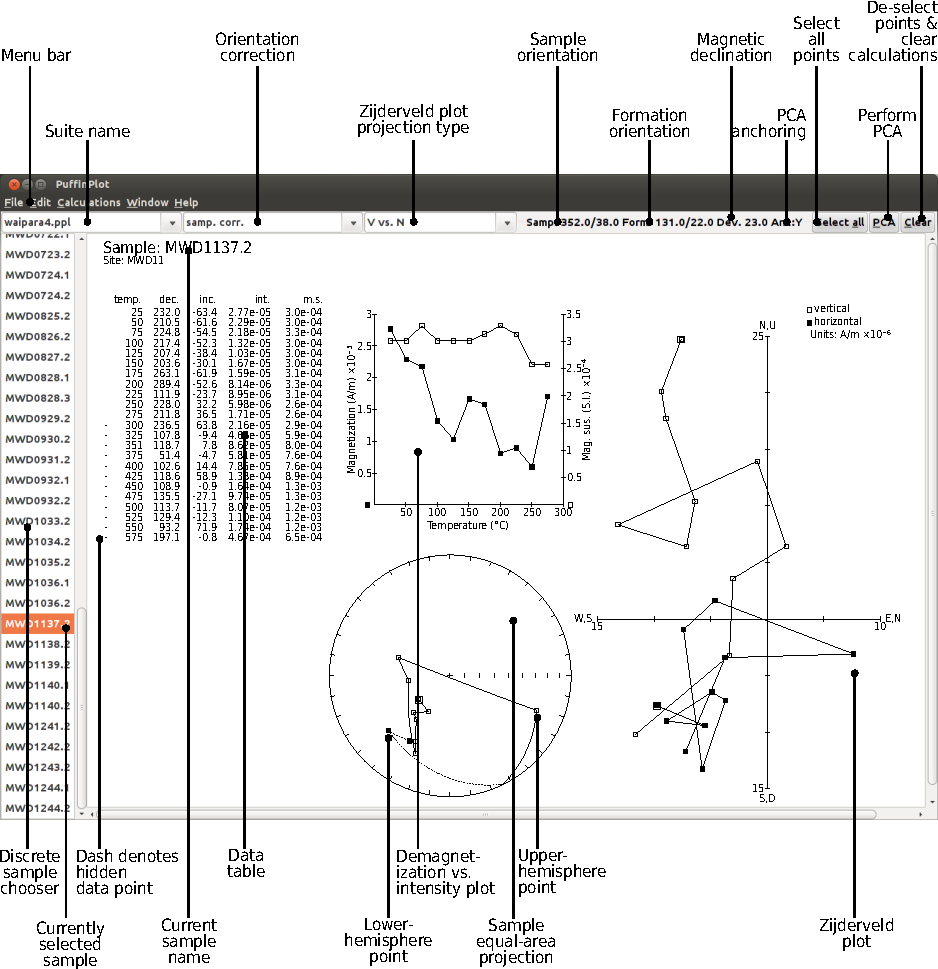
\includegraphics{figures/annot-scrnshot.pdf}
\else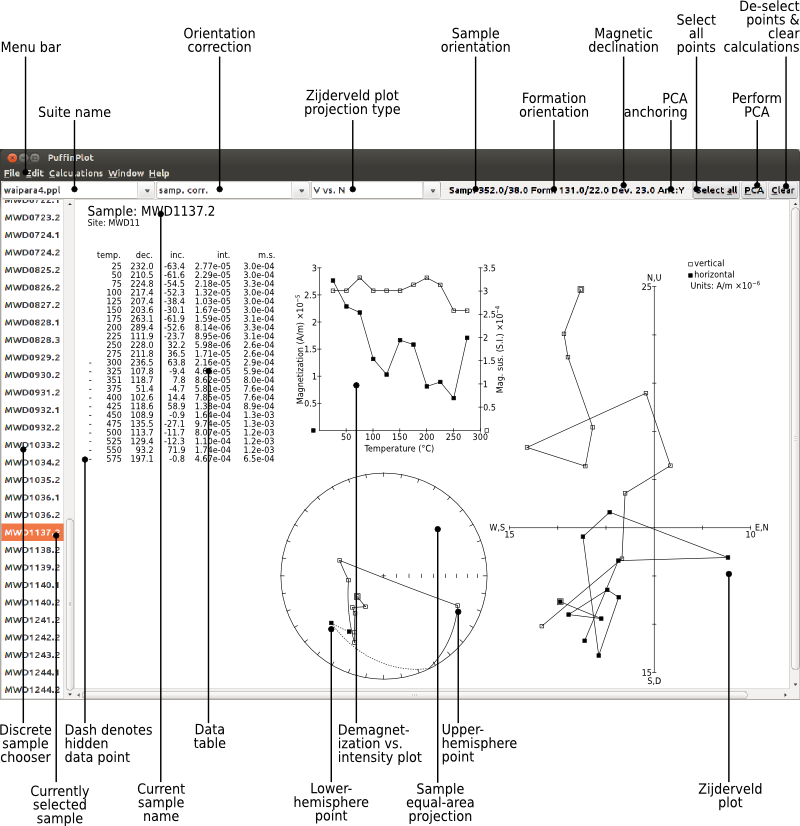
\includegraphics{figures/annot-scrnshot.png}
\fi
\caption{The main window of PuffinPlot with a discrete file loaded,
showing the default data plot layout. Data plots, information displays,
and controls are annotated. Note that several other data plots are
available, but are not shown by default, and that the layout may be
freely rearranged by the user. Data points above the 275\textdegree C
demagnetization step have been hidden.}
\end{figure}

\subsection{A tour of the main window}

Figure 1 shows an annotated screenshot of PuffinPlot's main window with
a discrete sample data file open. The bulk of the window is devoted to
the data display itself, and shows the four most popular data display
methods for palaeomagnetic data: a table, a Zijderveld plot, an
equal-area projection, and a demagnetization-intensity biplot (which
also shows an overlaid magnetic susceptibility plot). The plots are
interactive, in that individual data points may be selected by clicking
or by dragging a rectangle with the mouse.

To the left of the main plot display area is the sample chooser, which shows
a complete list of the samples within the suite, with the currently selected
sample highlighted. Multiple samples may be selected at once allowing
functions such as \caps{pca} calculation to be performed \emph{en masse}. If
a long core data file is loaded, the sample chooser is shown as a vertical
slider indicating depth rather than a list of sample names.

Above the main plot area is the toolbar, which gives convenient access
to some of the most frequently used facilities of the program. From left
to right, these are: choosers for the currently displayed data suite,
the orientation correction, and the Zijderveld projection type; displays
of the sample and formation orientations and magnetic declination; and
buttons for three of the most commonly performed actions.

At the top of the window is the menu bar, providing access to all the
program's functions in a hierarchical manner. On Mac OS, the menu bar is
at the top of the screen rather than the top of the window, and includes
an extra menu at the left, entitled \textsf{PuffinPlot}.

\subsection{Data model}

\begin{figure}[htbp]
\centering
\ifpdf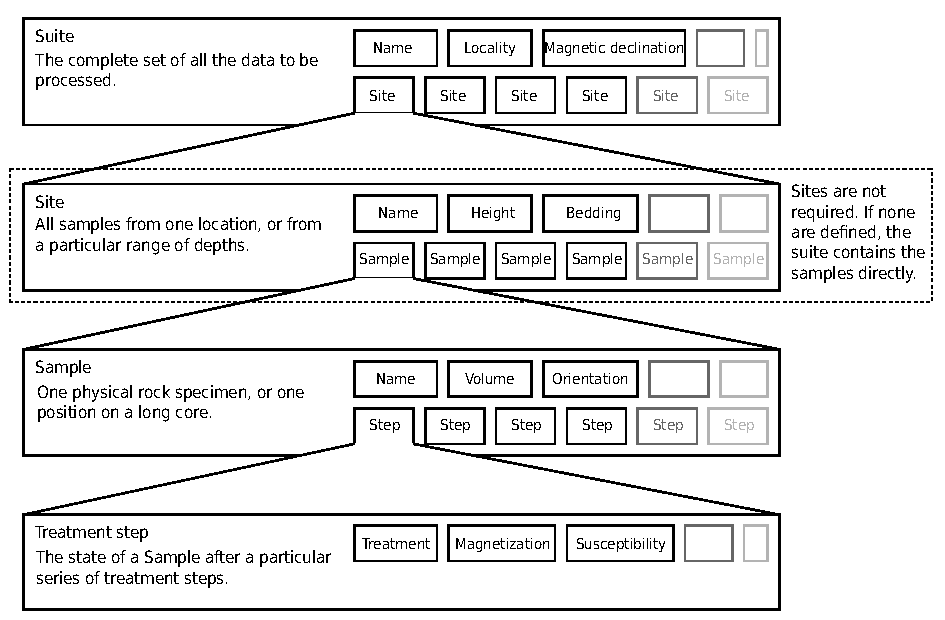
\includegraphics{figures/data-model.pdf}
\else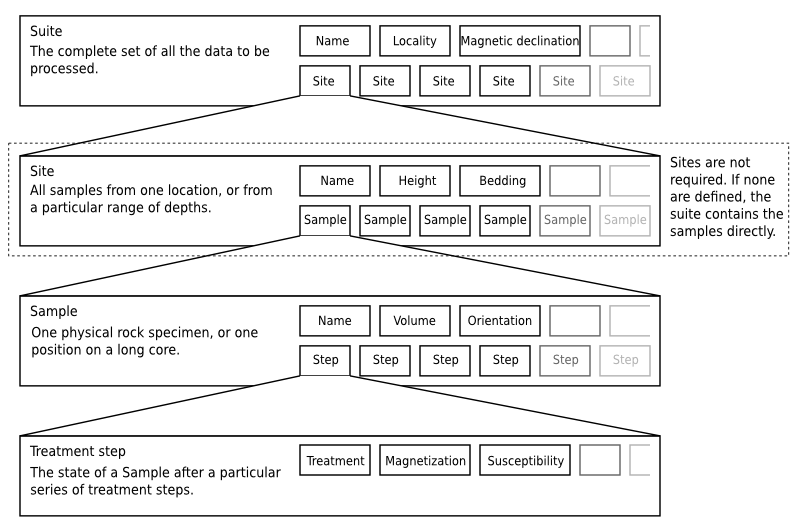
\includegraphics{figures/data-model.png}
\fi
\caption{PuffinPlot's hierarchical data model. Each layer (except the
lowest) contains multiple instances of the following layer.}
\end{figure}

PuffinPlot uses a hierarchical data structure, with higher levels
containing multiple instances of each lower level. The structure is
summarized in Figure 2. At the top is the \emph{suite}, which contains
all the data to be analysed as part of a particular study. For a
discrete specimen study, this will typically correspond to a section in
the field; for a long core study, it will correspond to a core. A suite
is initially created by opening one or more data files from a
magnetometer; it is saved as a file in PuffinPlot's own format. In a
discrete study, a suite contains multiple \emph{sites}. A site
corresponds to a set of samples taken from one spot in a section. A
site's associated data can include such things as bedding attitude and
stratigraphic height, as well as calculated parameters such as the mean
palaeomagnetic direction for all the samples at the site. For a long
core study, sites are not defined: samples are contained directly within
the suite.

Each site (or, for long core data, the suite) contains multiple
\emph{samples}. A sample corresponds to a small physical volume of rock.
For a discrete study, this will usually be a typical palaeomagnetic 25mm
cylinder or IODP cube sample. For long cores, it is the portion of the
core at a particular depth. The data associated with a sample consists
of information specific to this physical unit which does not change with
the application of demagnetization techniques --- for example, a sample
code or name (or, for long cores, a depth), the field orientation of the
sample, and its volume. For discrete samples this data can also include
a tensor representing anisotropy of magnetic susceptibility, which is
imported separately from an Agico kappabridge datafile and collated with
the magnetization data by matching the sample names. The sample can also
contain calculated parameters, such as a direction fitted by principal
component analysis, or a best-fitting great circle.

Each sample contains multiple \emph{demagnetization steps}. A
\emph{step} represents a sample at a particular point during the
treatment protocol. Its associated data thus includes details of the
treatment: the type (thermal, AF, IRM, etc.) and parameters
(temperature, field strength, etc.). The data also includes the state of
the sample itself --- most importantly, the measured magnetization
vector. For thermal studies, the magnetic susceptibility is usually also
recorded after every heating cycle, and is also stored as part of the
step.

\subsection{Main window features}

This section describes the parts and functions of the main PuffinPlot
window, as shown in Figure 1.

\subsubsection{Plot area}

The plot area is the largest part of the window, and plots the data for
the current sample using various plots. By default, four plots are
shown: a demagnetization-intensity biplot, a Zijderveld plot, an
equal-area projection, and a table of demagnetization steps. The plots
can be moved and resized (see
in\{section\}{[}sec:manual-change-layout{]}). Other plots are also
available, and the preferences window can be used to control which plots
are displayed (see in\{section\}{[}sec:manual-preferences{]}).

\subsubsection{Sample chooser}

The sample chooser sits at the leftmost edge of the main window, and
allows you to change the current sample (the one for which data is
plotted) and the set of selected samples (most of PuffinPlot's functions
operate on the currently selected samples). Often, the set of selected
samples will consist only of the current sample.

The sample chooser takes two forms, depending on whether the current
suite of data is for discrete samples or for a continuous long core
measurement.

\paragraph{Using the discrete sample chooser}

The discrete sample chooser shows the names of the samples in the current
suite. The selected sample or samples are highlighted in a different colour.
If more than one sample is selected, the first of them is displayed in the
main plot area.

To select a single sample, click on its name. To select a contiguous range of
samples, click at one end of the range, then hold down \ppcmd{Shift} while
clicking at the other end of the range. To select multiple, non-contiguous
samples, hold down \ppcmd{Ctrl} while clicking. To select all samples, press
\ppcmd{Ctrl-A}.

\paragraph{Using the continuous sample chooser}

The continuous sample chooser is a vertical grey bar representing the total
length of the measured core, striped with horizontal white lines representing
the individual measurements at each depth. (If there are too many
measurements for all the requisite white lines to be displayed, they are
omitted.) A black triangle and line show the current depth. The selected
samples are denoted with orange highlighting.

To select a single depth, click on the appropriate part of the sample
chooser. To scroll rapidly through a range of samples, click and drag the
mouse along the sample chooser. To select a range of samples, hold down
\ppcmd{Shift}, then click, drag, and release the mouse on the chooser.

\paragraph{Keyboard shortcuts for sample selection}

Use \ppcmd{Ctrl-B} and \ppcmd{Ctrl-N} to change the current sample. Use
\ppcmd{Ctrl-A} to select all the samples in the current suite. You can also
use the up and down arrow keys to change the sample.

\subsubsection{\label{sec:manual-toolbar}Toolbar}

The toolbar displays various data and provides several controls.
From left to right, these are:

\begin{description}

\item[Suite chooser.] This shows the name of the current suite of
data. If more than one suite of data has been opened, the suite chooser
allows you to switch between them.

\item[Orientation correction chooser.] This chooser allows you to
choose whether data is displayed in laboratory co-ordinates
(\ppcmd{uncorrected}), in field co-ordinates, corrected for sample orientation
(\ppcmd{samp. corr.}), or in tectonic co-ordinates, corrected for both
sample orientation and bedding orientation (\ppcmd{form. corr.}).

\item[Zijderveld projection type.] This chooser controls the vertical
projection used in the Zijderveld plot. The {\em y} axis always corresponds
to the vertical direction; the chooser controls the {\em x} axis, which may
correspond to North (\ppcmd{V vs. N}) or East (\ppcmd{V vs. E}). The third
option, \ppcmd{V vs. H}, projects each data point separately, in the plane
containing itself and the origin; this is sometimes referred to as a
`modified Zijderveld' plot.

\item[Sample orientation] (\ppcmd{Samp}). The first number is the
azimuth of the sample orientation; the second is its dip. For a long core,
all these values will usually be 0 and 90 respectively throughout the core.

\item[Formation orientation] (\ppcmd{Form}). The first number is the
dip direction of the bedding; the second in the dip magnitude.

\item[Magnetic declination] (\ppcmd{Dev}). This is the angle between
magnetic north and true north at the sampling site.

\item[Select all] selects all the points in the current sample.

\item[\caps{Pca}] performs principal component analysis for the
selected points of all the selected samples.

\item[Clear calculations] de-selects all the points in all the
selected samples, and clears the results of any calculations done on them,
such as \caps{pca} or great-circle analysis.

\end{description}

\section{Detailed usage}

This section gives a methodical account of PuffinPlot's features.

\subsection{Catalogue of functions}

This section lists all the items in PuffinPlot's menus, giving a brief
description of the functionality associated with each one.

\subsubsection{File menu}

This menu contains functions connected with opening, closing, and
saving files.

\begin{menuitemlist}

\item[File\submenu Open…] loads one or more files of demagnetization data into
  PuffinPlot as a new suite. See section~\ref{sec:manual-file-types} for
  details of supported filetypes.

\item[File\submenu Open recent file] is a submenu which
contains the names of the last eight files which have been opened in
PuffinPlot, allowing them to be opened again with a single click.

\item[File\submenu Save] saves the current suite as a PuffinPlot file. If
the suite was opened from a PuffinPlot file or if it has been previously
saved as a PuffinPlot file, it will immediately be saved to that file. If no
PuffinPlot file is associated with this suite yet, a standard ‘save file’
dialog box will prompt yo for a file name and location.

\item[File\submenu Save as…] allows you to save the current suite to a
different filename or location.

\item[File\submenu Close] closes the current suite, removing it from
PuffinPlot's data display.

\item[File\submenu Export data] is a submenu allowing the export of
various kinds of data to \caps{csv} files.

\item[File\submenu Export data\submenu sample calculations…] saves a file
containing all the data associated with individual samples.
Table~\ref{tbl:manual-export-sample} describes the fields which make
up the file.

\end{menuitemlist}

\bibliographystyle{plainnat}
\bibliography{manual}

\end{document}
